\documentclass{article}
\usepackage[fleqn]{amsmath}
\usepackage{amssymb,graphicx,color,graphicx,slashed, microtype, parskip, enumitem, extarrows, needspace}
%\usepackage[utf8x]{inputenc}
\usepackage[top=1.5cm, bottom=1.5cm, right=6cm, left=1.5cm, heightrounded, marginparwidth=5cm, marginparsep=0.5cm]{geometry}

\hbadness = 10000
\hfuzz=100pt 
    
\usepackage{marginnote}
\renewcommand*{\marginfont}{\footnotesize}

\usepackage{hyperref}
\hypersetup{colorlinks=true, urlcolor=NavyBlue, bookmarksdepth=3}

\makeatletter\newcommand{\@minipagerestore}{\setlength{\parskip}{\medskipamount}}\makeatother

% =============== Index ===========================

\usepackage[nonewpage]{imakeidx}
\makeindex

% =============== Color Definitions ===============
    
\usepackage[svgnames]{xcolor}
\colorlet{ColorTitle}{Black}
\colorlet{ColorSectionName}{Black}
\colorlet{ColorBoxFG}{Gray}
\colorlet{ColorBoxText}{Black}
\colorlet{ColorBoxBG}{White}


% =============== Title Style ===============
    
\usepackage{titling} % Allows custom title configuration
    
\newcommand{\HorRule}{\color{ColorTitle}\rule{\linewidth}{1pt}} % Defines the gold horizontal rule around the title
    
\pretitle{
    \vspace{-50pt} % Move the entire title section up
    \HorRule\vspace{9pt} % Horizontal rule before the title
    \fontsize{27}{36}\usefont{OT1}{phv}{b}{n}\selectfont
    \color{ColorTitle} % Text colour for the title and author(s)
}
    
\posttitle{\par\vskip 15pt} % Whitespace under the title
    
\preauthor{\fontsize{17}{0}\usefont{OT1}{phv}{m}{n}\selectfont\color{ColorTitle}} % Anything that will appear before \author is printed
    
\postauthor{\par\HorRule}

\newcommand{\COURSENAME}{\href{http://phyw.people.ust.hk/teaching/PHYS2022-2015/}{\textcolor{black}{PHYS 2022}}}
\newcommand{\YW}{\href{http://phyw.people.ust.hk/}{\textcolor{black}{Yi Wang}}}
\newcommand{\PHYS}{\href{http://physics.ust.hk}{\textcolor{black}{Department of Physics}}}
\newcommand{\HKUST}{\href{http://www.ust.hk/}{\textcolor{black}{HKUST}}}
\author{\COURSENAME, \YW, \PHYS, \HKUST}

\date{}

% =============== Section Name Style ===============
    
\usepackage{titlesec}
    
\titleformat{\section}
    {\fontsize{15}{20}\usefont{OT1}{phv}{b}{n}\color{ColorSectionName}}
    {\thesection}{1em}{}
    %[{\vspace{0.2cm}\titlerule[0.8pt]}]
    
\titleformat{\subsection}
    {\fontsize{14}{20}\usefont{OT1}{phv}{m}{n}\color{ColorSectionName}}
    {\thesubsection}{1em}{}
    
\titleformat{\subsubsection}
    {\fontsize{12}{20}\usefont{OT1}{phv}{m}{n}\color{ColorSectionName}}
    {}{0em}{}
      
\setcounter{secnumdepth}{4}
        
% =============== Box Style ===============
    
\usepackage[most]{tcolorbox}
    
\newtcolorbox{tbox}[1]{
    colback=ColorBoxBG, colframe=ColorBoxFG, coltext=ColorBoxText,
    sharp corners, enhanced, breakable, parbox=false,
    before skip=1em, after skip=1em,
    title={#1}, fonttitle=\usefont{OT1}{phv}{b}{n}, 
    attach boxed title to top left={yshift=-0.1mm}, boxed title style={sharp corners, colback=ColorBoxFG, left=0.405cm},
    rightrule=-1pt,toprule=-1pt, bottomrule=-1pt
}

\newtcolorbox{mtbox}[1]{
    colback=ColorBoxBG, colframe=ColorBoxFG, coltext=ColorBoxText,
    sharp corners, enhanced, breakable, parbox=false,
    before skip=1em, after skip=1em,
    title={#1}, fonttitle=\usefont{OT1}{phv}{b}{n},
    attach boxed title to top left={yshift=-0.1mm}, boxed title style={sharp corners, colback=ColorBoxFG, left=0.15cm},
    rightrule=-1pt,toprule=-1pt, bottomrule=-1pt, 
    left=0.5em
}

% =============== tikz has to be loaded after xcolor
\usepackage{tikz}

\newcommand*\enumlabel[1]{\tikz[baseline=(char.base)]{
			\node[shape=rectangle,inner sep=2pt,fill=ColorBoxFG] (char) 
			{\fontsize{7}{20}\usefont{OT1}{phv}{b}{n}{\textcolor{ColorBoxBG}{#1}}};}}

% =============== Useful shortcuts ===============

\newcommand\wref[1]{{\hypersetup{linkcolor=white}\ref{#1}}}  

\newcommand{\textbox}[2]{
    \begin{tbox}{#1}
        #2
    \end{tbox}
}

\newcommand{\mtextbox}[2]{\marginnote{
    \begin{mtbox}{#1}
        #2
    \end{mtbox}}
}

\newcommand{\mnewline}{\vspace{0.5em}\newline}

\newcommand{\titem}[1]{
    \begin{itemize}[label=\color{ColorBoxFG}$\blacktriangleright$, leftmargin=0mm, labelsep=0.27cm, topsep=0.5em
        %, itemsep=1ex
        ]
        #1
    \end{itemize}
}

\newcommand{\mtitem}[1]{
    \begin{itemize}[label={\color{ColorBoxFG}$\blacktriangleright$}, leftmargin=0mm, labelsep=1mm, topsep=0.5em
        %, itemsep=1ex
        ]
        #1
    \end{itemize}
}

\newcommand{\itembox}[3]{
    \begin{tbox}{#1}
        #2
        \titem{#3}
    \end{tbox}
}

\newcommand{\mitembox}[3]{
    \marginnote{
    \begin{mtbox}{#1}
        #2
        \mtitem{#3}
	\end{mtbox}
    }
}

\newcommand{\tenum}[1]{
    \begin{enumerate}[label=\protect\enumlabel{\arabic*}, leftmargin=0mm, labelsep=0.265cm, topsep=0.5em
        %, itemsep=1ex
        ]
        #1
    \end{enumerate}
}

\newcommand{\enumbox}[3]{
    \begin{tbox}{#1}
        #2
        \tenum{#3}
    \end{tbox}
}

\newcommand{\twocol}[5]{
    \begin{minipage}[t][][b]
        {#1\textwidth}
        #4        
    \end{minipage}
    \hspace{#2\textwidth}
    \begin{minipage}[t][][b]
        {#3\textwidth}
        #5
    \end{minipage}
}

\newcommand{\cg}[2]{
    \begin{center}
        \includegraphics[width=#1\textwidth]{#2}
    \end{center}
}

\newcommand{\tbar}{
    ~\newline
    {\color{ColorBoxFG}
    \hbox to 0.15\textwidth{\leaders\hbox to 5pt{\hss  \hss}\hfil} 
    \hbox to 0.7\textwidth{\leaders\hbox to 5pt{\hss . \hss}\hfil}}
    \mnewline
}

% =============== Filter unwanted warnings
\usepackage{silence}
\WarningsOff[tcolorbox]
\hbadness=1000000


\usepackage{5_fig/modiagram}
\graphicspath{{5_fig/}}
\title{第五章\ 原子物理}
\usepackage{ctex}

\begin{document}

\maketitle

\textbox{费曼的问题}{
    费曼在他的讲座开头问了以下这个问题:
    \begin{quote}
        如果在一个大灾变里,所有科学知识全部被毁灭,但是仅有一句话可以被传到下一代生物。哪句话可以在尽可能少的话里传达最多的信息?
    \end{quote}
    他的答案是:
    \begin{quote}
        所有物质都是由原子构成的。
    \end{quote}
    这句话并不完全正确。例如:E\&M电磁波被当成物质的一种,但是它并不是由原子组成的(由量子组成)。暗物质也不是由传统原子组成的,暗物质长得也不像原子。无论如何,我们熟悉的世界确实是由原子组成的。 
    \marginnote{
        用现代的眼光看,\ref{item:atom-chem}、\ref{item:atom-size}、\ref{item:atom-evid}都很容易。这是因为运用扫描隧道显微镜,人们可以直接地看见并操控原子。但是在150$\sim$200年前,这些特征是如何从科学方法中得知的?更严谨的来说,他们不是现代物理学的一部分。但是普通物理学又没有完全覆盖这些特征,所以我们在这里列出了这些特征。
    }
    我也同意这句话应该被传下去。
    \tcblower
    这句话我们是怎么知道的、为什么要知道、对世界的影响又是什么?这将是这部分的重点。更详细的来说,我们会解释:
    \tenum{
        \item 原子论是怎么在化学里产生的?\label{item:atom-chem}
        \item 我们怎么知道原子的大小?\label{item:atom-size}
        \item 我们能否找到原子存在的直接证据?\label{item:atom-evid}
        \item 原子是怎么稳定的?量子力学是怎么拯救世界的?\label{item:atom-quantum}
        \item 原子的化学性质从何而来?\label{item:atom-chem-nature}
    }
    \mtextbox{油膜法}{
        原子(分子)的大小也可以用油膜法测定。富兰克林(1757)注意到石油可以在大片水域扩散。在水上的这层油的薄膜可以跟单独一层分子一样薄。但是,这么大的面积是很难测量的。能否让油的量变少呢?
        \tcblower
        朗缪尔(1917)用酒精溶解油酸。在水里面滴一滴这个溶液。 酒精被水溶解,油酸在水的表面扩散。这个面积可以在实验室里测量。
    }
}

\section{我们是怎么知道物质是由原子组成的?}

2000年前,原子论由古希腊(及其他古文明)提出。但是当时原子论是基于哲学的猜测与极少的科学依据。科学的量子论从19世纪开始。

\textbox{道尔顿的多重比例定律\index{道尔顿的多重比例定律}}{
    道尔顿(1808)注意到碳可以以两种不同的方式与氧结合形成氧化物。碳的量不变,两种氧化物需要氧的量之比是1:2--一个由两个小整数组成的比例。 

    这个观察是巧合吗?道尔顿测试了其他(可以组成至少两个化合物的)元素组合。他注意到了相似的特性:一个元素的量不变,不同化合物所需的另一种元素的量是一个小整数的比值。
    \tcblower
    这样的观察需要一个解释。
    \mtextbox{多重比例定律是一个惊喜吗?}{
    物理学家的一大才能是去分辨哪些科学观察是普通的、哪些是惊人的并且会导致历史性突破的。
    对现在的人来说多重比例定律是普通的,因为我们都知道物质是由原子构成的,但是在道尔顿的时期这个却是惊人的。如果我们不知道物质都是原子构成的,那么合并碳和氧就跟在面包上涂黄油一样--一块面包上黄油的量是可以持续变化的。然而道尔顿的发现表明了--只有两种面包:涂有5克黄油的和涂有10克黄油的。不存在涂有6克黄油的面包。难道这个不是一个惊人的发现吗?
    \tcblower
    你可能会觉得这里的讨论很熟悉--它与光子和光电效应的讨论相似--只不过这个更基础。理论上来说,物质或光子是由量子组成的是一样惊人的。它们都有波的特性也是一样的惊人。只是在实践中,某些属性比其他属性更容易观察。}
    道尔顿指出原子论可以很好的解释这一发现。比如说,在碳和氧的例子中,一个化合物是一氧化碳,另一个是二氧化碳。那么氧的量的比很显然是1:2。另一方面来说,如果物质没有基本组成部分,那么这个比例就不会是简单的。这是原子论的第一个科学依据。
}

我们现在知道原子存在了。那么它们的性质是什么呢?气体的动力学理论是为了解释热。对于原子论来说,接下来的问题是:(一)原子运动的有多快?(二)原子有多大?

在本章的其余部分,我们将关注数量级估计,而不注意系数。当我们在等式中使用“$\sim$”时,我们已经忽略了一阶系数。而且我们假设室温与1atm的气压。并且我们不会关注原子和分子之间的差别。

\textbox{原子在气体中的移动速度有多快?\index{原子:热运动速度}}{
    1654年,马德堡半球实验证实了空气有巨大的压力 -- 16匹马才能分开两个直径为50厘米、中心为真空的半球。大气压力为$1\mbox{ atm}\sim 10^5 \mbox{pa}$。这在当时是很难想象的因为人们竟然感受不到如此强大的压力;但是又是很容易想象的因为有几公里厚的气体在我们头上,它们也受引力作用。

    在气体的动力学理论中,压力是由原子相互碰撞(或容器)产生的。对于理想气体
    \begin{align}
        P= \frac{1}{3} n m v^2~,
    \end{align}
    $m$为单独一个原子的质量;$n$为原子的数密度;$v$为速度的均方根。对于数量级分析,我们把$v$当成原子随机运动的典型速度。
    
    气体的密度为
    \begin{align}
        \rho = n m \sim 1\mbox{kg}/\mbox{m}^3~,
    \end{align}
    我们可以得到\marginnote{或者我们可以用气体的比热容$C_V \sim k_B/m \sim 1000 \mbox{J}/\mbox{kg}/\mbox{K}$以及$k_B T \sim \frac{1}{2} m v^2$来求出相同的速度。}
    \begin{align}
        v = \sqrt{3P/\rho} \sim 10^3 \mbox{m}/\mbox{s}~.
    \end{align}
    原子运动速度很快!他们得面对压力迅速地移动。
}

\textbox{原子在气体里是自由运动的吗?\index{原子:平均自由路径}}{
    不一直是。他们会相互碰撞。那么原子可以不碰撞地自由运动的典型距离$L$是什么呢?$L$也被称为平均自由路径。

    我们用具有有限并固定直径$d$的硬球来模拟原子。 
    \marginnote{$L$可以用以下方法来估算:将一个长度为 $L$ 且面积为 $A$的(原子)盒子挤压到一层原子,该层可以填充大部分面积$A$。盒子里原子的数量是$N=nLA$。为了将原子压缩到一层,原子的总横截面为$Nd^2 \sim A$。因此$L \sim 1/ (d^2 n)$.}
    那么平均自由路径就是 
    \begin{align}
        L \sim 1/ (d^2 n)~.
    \end{align}
    \tcblower

    可不可能用(不需要像原子一样小的长度)的简单实验来测量$L$ ?麦克斯韦(1859)提出了用气体的粘度来测量$L$。这里我们提供一个简化的教学论点。

    \begin{center}
        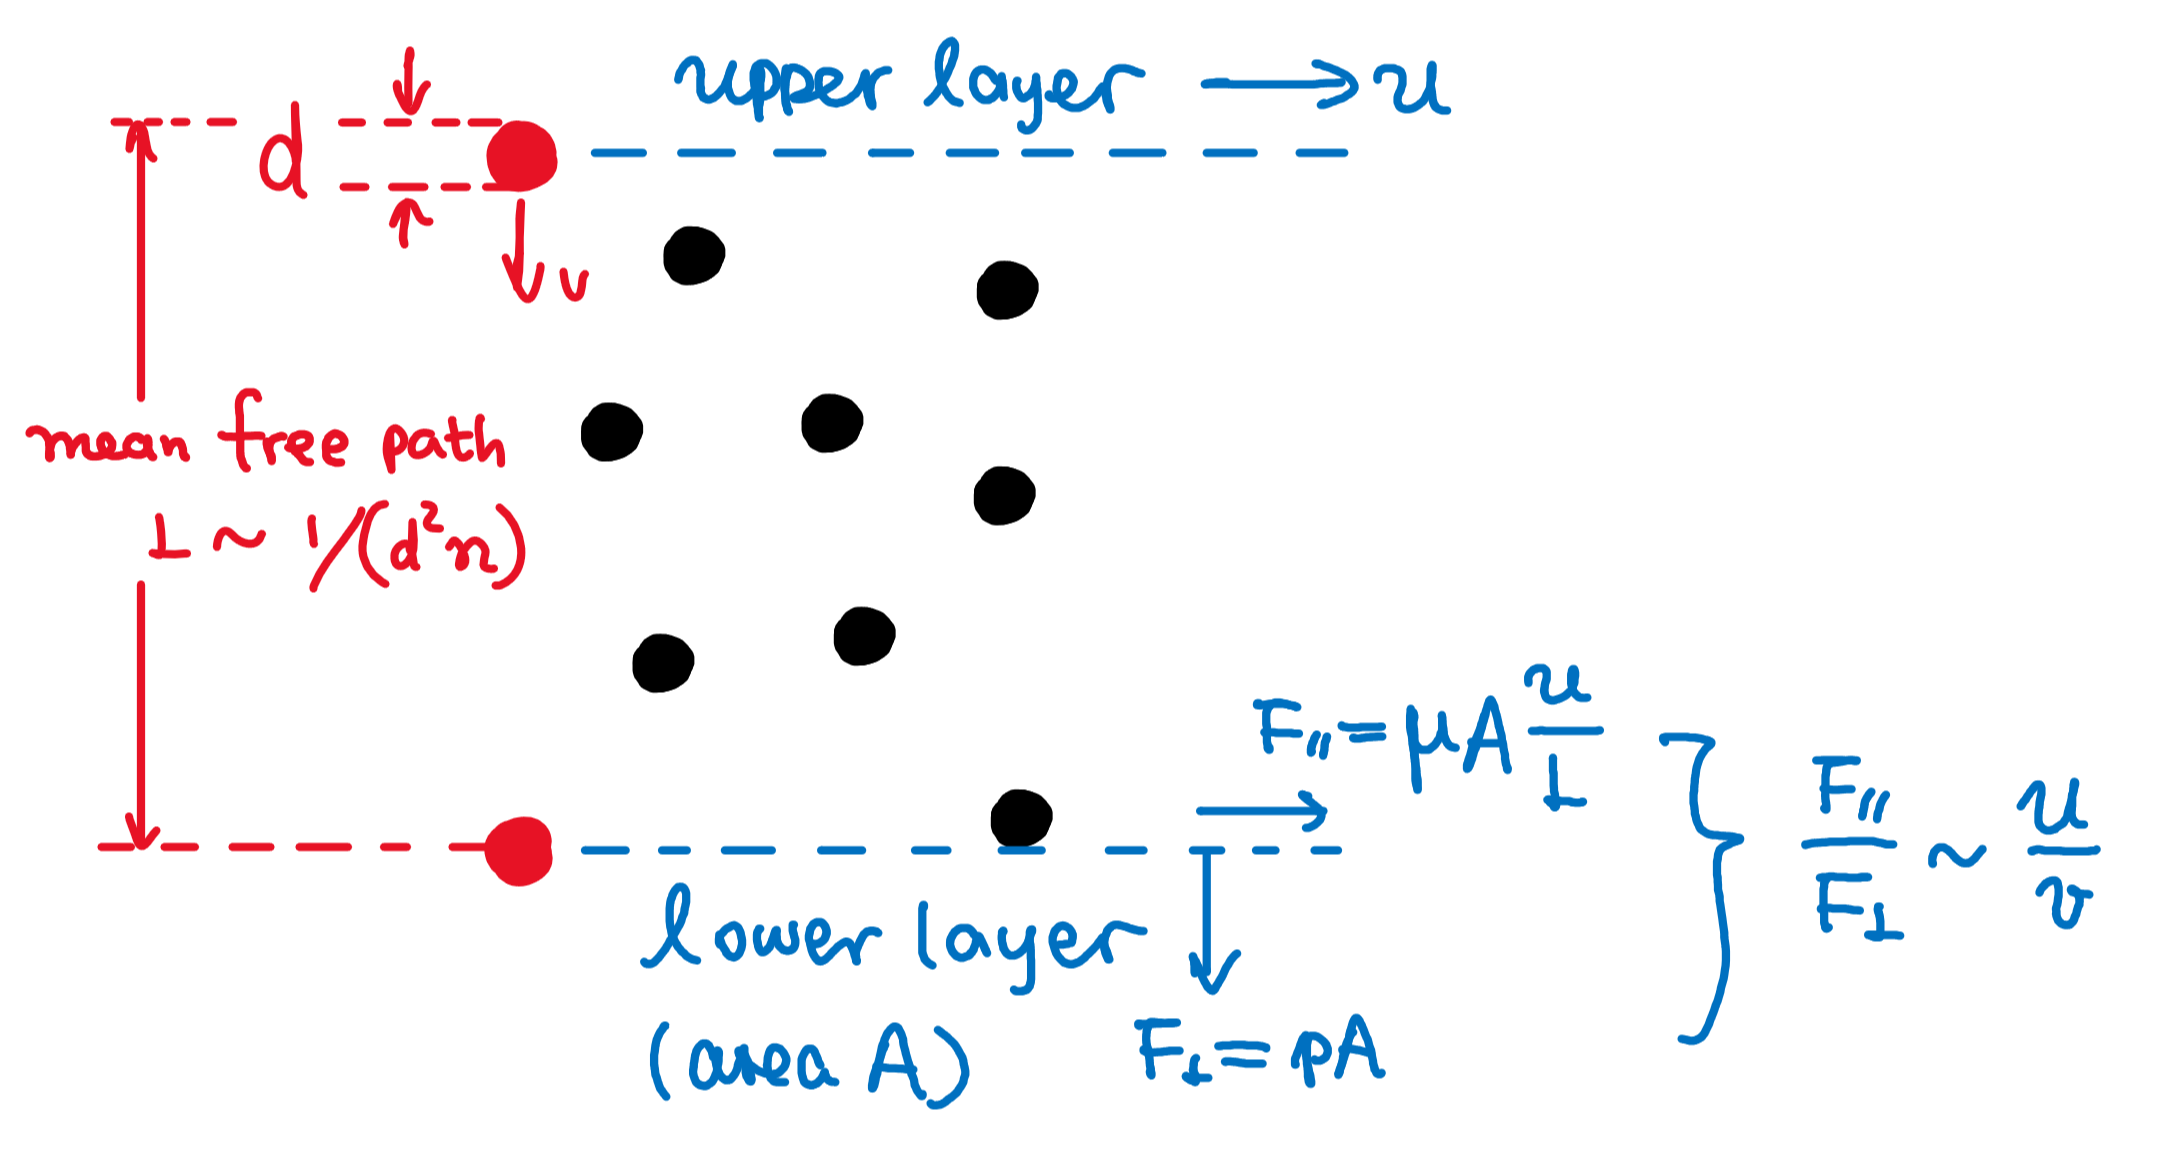
\includegraphics[width=0.7\textwidth]{viscosity}
    \end{center} 

    气体的粘度$\mu$的定义为
    \begin{align}
        F_{\parallel} = \mu A u / y~,
    \end{align}
    $A$为每一层的面积;$y$为每层之间的距离。然后$u$就是 层间运动速度的非随机部分。空气的粘度为$\mu \sim 10^{-5} \mbox{kg} / \mbox{m} / \mbox{s}$。
    
    上图中,我们有两层分开$y=L$的气体。平均来说,力通过一阶碰撞从上层传递到下层。我们知道垂直于下层的力$F_\perp = p A$ 与$F_{\parallel}$的关系式为
    \begin{align}
        \frac{F_\parallel}{F_\perp} \sim \frac{u}{v}~, 
    \end{align}
    因为它们来自于相同的碰撞(冲力具有相同的碰撞时间)。

    把以上的方程结合,原子的平均自由路径为
    \begin{align}
        L \sim \frac{\mu v}{p} \sim 10^{-7} \mbox{m}~.
    \end{align}
}

人们可以在无法看到单个原子(当时)的情况下推断出原子的速度和平均自由路径。那么我们还可以求出原子的大小吗?

\textbox{原子的大小\index{原子:大小}}{
    罗什米特通过一个简易的实验(基于之前提到的平均自由路径)求出了原子的大小。当气体在低温液化,它的体积缩小了约1000倍(当液体固化体积变化不大)。液体和固体的数密度$\tilde n$可以估算为
    \begin{align}
        \tilde n \sim d^{-3} \sim 1000 n \sim 1000 d^{-2} L^{-1}~.
    \end{align} 
    这里我们假设原子在液体和固体中紧密排列。因此一个原子的大小可以估算为
    \begin{align}
        d \sim 10^{-3} L \sim 10^{-10} \mbox{m}~.
    \end{align}
}

19世纪末,原子论已经比较成功了。正如威廉汤姆森爵士在1889年记载,原子论
% Sir William Thomson, Popular Lectures and Addresses, Vol. I., London, 1889, p. 148.
\begin{quote}
    ...分别建立在光的波动理论、接触电现象、毛细吸引力和气体动力学理论的基础上。它们都能证明普通物质的原子或分子一定是直径为1/10,000,000厘米,或是l/10,000,000厘米到 l/100,000,000厘米。
\end{quote}

但是,原子论还在接受质疑(比如说马赫的)因为没有人真的见过一个原子。那么原子论只是一个用来解释实验的“有效的”理论吗?还是说原子真的是\emph{真实}世界的基本组成部分?

\textbox{(可选)布朗运动\index{布朗运动}}{
    1827年,
    \marginnote{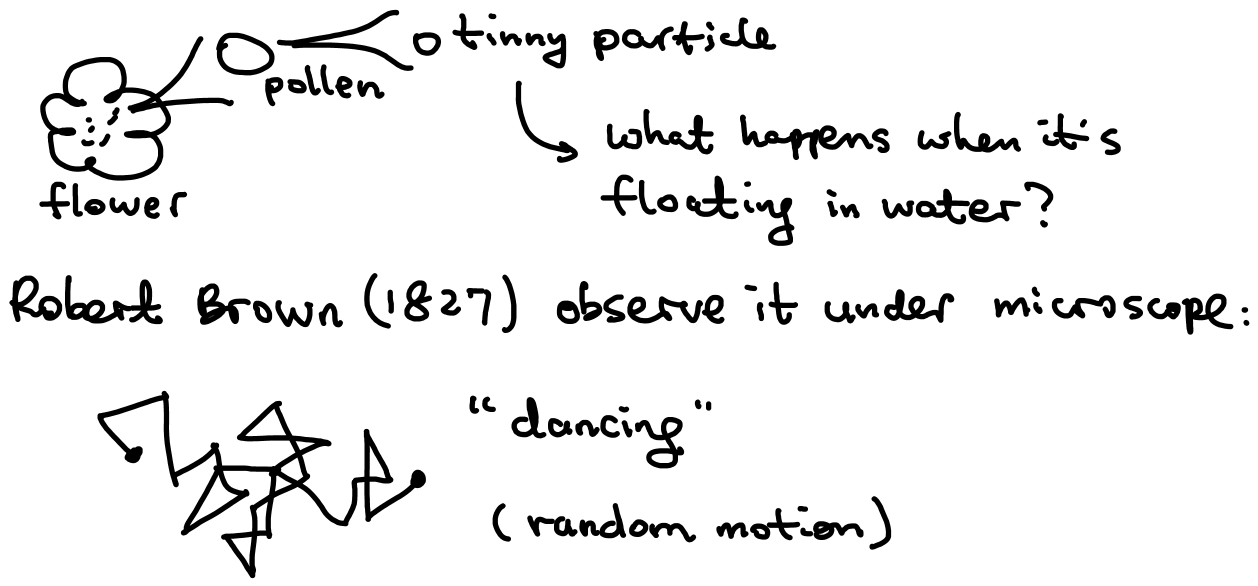
\includegraphics[width=0.4\textwidth]{brownian}} 
    罗伯特布朗观察到花粉中微笑的粒子在水里“跳舞”。爱因斯坦在1905年用分子的运动解释了这些跳舞的粒子:我们可以看到他们的直接作用。这里我们用朗之万的随机微分方程(1908)来描述爱因斯坦的想法。
    
    花粉的粒子持续被水分子碰撞。粒子的速度满足一下朗之万方程\index{朗之万方程}
    \begin{align}
        M \frac{dv}{dt} = -\lambda v + f(t)~,    \label{eq:lang}
    \end{align}
    这里
    \titem{
        \item 参数$M$是粒子的质量。
        \item 参数$\lambda$描述了一个摩擦力(在水中的耗散)。这个耗散可以用一个重球在深水中的最终速度来测量。
        \item 函数$f(t)$是分子对粒子的随机的力。这个随机的力可以用白噪声来模拟:
        \begin{align}
          \label{eq:f_rand}
          \langle f(t) \rangle = 0~, \qquad 
          \langle f(t) f(t') \rangle = \Lambda \delta(t-t')~.
        \end{align}
        相似于量子力学中的符号,这里的$\langle \cdots \rangle$ 代表取平均值。 
        \marginnote{非常近似的,这些随机的力是互相独立的。因此在不同时间的随机力之间没有相关性。但是同时,“同”一个随机力跟自己有相关性。这就是为什么$\langle f(t) f(t') \rangle$与$\delta(t-t')$成正比。参数$\Lambda$ 表征粒子的波动的速度。}
        $\Lambda$可以用以下方法测量:给定一组最初在重合位置的粒子,由于波动,粒子扩散。我们可以通过该组粒子的扩散速度获得$\Lambda$。
    }
    朗之万方程\eqref{eq:lang}可以用“常数的变化”方法来求解:
    \begin{align}
        \label{eq:sol_lang}
        v(t) = v_0 e^{-\frac{\lambda}{M} t}
        + \frac{1}{M}  \int_0^{t} dt_1 f(t_1) e^{-\frac{\lambda}{M}(t-t_1)} ~.      
    \end{align} 
    因此,
    \begin{align}
        \langle v(t) \rangle = \langle v_0 \rangle e^{-\frac{\lambda}{M} t}~.
    \end{align}
    \begin{align}
        \label{eq:lang_v2}
        \langle v^2(t) \rangle & = \langle v_0^2 \rangle e^{-2\frac{\lambda}{M} t}
        + \frac{1}{M^2} \int_0^t dt_1 \int_0^t dt_2 
        e^{-\frac{\lambda}{M}(t-t_1)} e^{-\frac{\lambda}{M}(t-t_2)}
        \langle f(t_1) f(t_2) \rangle
        \nonumber\\ &
        = \langle v_0^2 \rangle e^{-2\frac{\lambda}{M} t}
        + \frac{\Lambda}{2M\lambda} \left ( 1-e^{-2\frac{\lambda}{M} t} \right )~. 
    \end{align}
    过了很长的时间$t$,指数抑制项(关于初始条件的记忆)消失了。所以$\langle v(t) \rangle$消失了,然后\marginnote{注意$\frac{1}{2}  M\langle v^2(t) \rangle = \frac{1}{2} k_B T$。因此这是个对玻尔兹曼常数的直接测量。1908年,佩林进行了这个测量。}
    \begin{align}
    \label{eq:lang_v2_infty}
        \frac{1}{2}  M\langle v^2(t) \rangle & = \frac{\Lambda}{4\lambda}~. 
    \end{align}
    我们计算了这个粒子的平均动能。注意这个能量应该在统计上与水分子的动能一样,因为不然的话这些粒子会把能量传递给水分子然后失去能量(均分定理)。与每单位体积的总内能相比,我们知道存在多少个原子,也就知道了他们的大小。
}

\needspace{0.3\textheight}
\mtextbox{距离阶梯}{
    我们接触了3种测量原子大小的方法。每个方法都建造了一个从人类可接近的尺度到微观尺度的距离阶梯。
    \mtitem{
        \item 油膜:通过油醇溶液。
        \item 动力学理论:通过三个大或小的数:空气压力、粘度、从气体到液体的冷凝率。
        \item 布朗运动:通过花粉里微小粒子的运动。
    }
    \tcblower
    距离阶梯是接触我们无法达到距离的一个重要的技术。这对大距离也有帮助。比如说测量天文学和宇宙学里的距离。
}
\textbox{(可选)波动和耗散:爱因斯坦的另一个等价物\index{涨落耗散定理}}{
    对布朗运动的解释是另一爱因斯坦式的发现。让我们更仔细地看布朗运动里的两个可测量的数:$\Lambda$代表波动的强度; $\lambda$代表耗散的速度。第一眼看他们是毫无联系的,但是爱因斯坦注意到他们有同一个来源。

    为什么存在耗散?大尺度的来讲,它们是来源于粘度或者摩擦。但是在小尺度来讲,想象你是那个粒子,你一旦往前跑,更多的分子会打到你的脸而不是你的后背。因此随机力倾向于阻止你的运动。这就把波动和耗散联系到了一起。

    这个观察可以概括为统计物理学中的涨落耗散定理。它有很多的应用。比如说,电阻器的热噪声(约翰逊-奈奎斯特噪声)。这个讨论甚至能(很松的)应用到社会学上 -- 一个富有创造力的社会(更多的波动)经常缺少执行能力(更多的耗散),所以同时拥有创造力和执行能力是个挑战。
}

\section{氢原子} \label{sec:atom-hydrogen}

我们现在理解了物质是原子组成的。让我们继续研究原子的性质。从最简单的开始:氢原子。

\subsection{观察方面}

牛顿之后,很多科学家研究了光谱。因为物质是原子组成的,物质发射或吸收的光也(一般)会被原子发射或吸收。那么我们可不可以从光谱的研究里学习原子的性质呢?
\marginnote{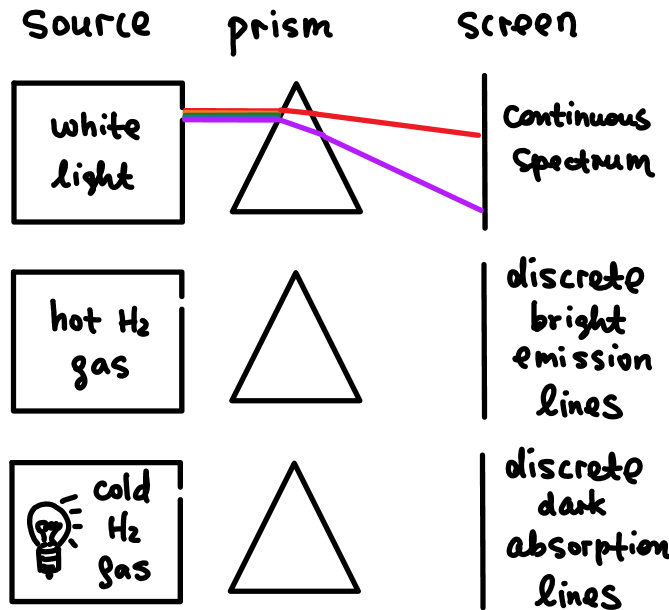
\includegraphics[width=0.35\textwidth]{hlines}}

% reference: http://web.mit.edu/spectroscopy/history/history-classical.html
\textbox{光谱学的发展\index{原子:光谱学}}{
    \titem{
        \item 1666年,牛顿:用棱镜将阳光形成光谱。
        \item 1814年,夫琅和费:太阳光谱中的暗线。
        \item 1817-1823年,夫琅和费:月球、金星、火星的光谱在太阳光谱的相同位置有一些暗线。它们也有一些新的暗线。
        \item 1826年,赫歇尔和塔尔博特:发射光谱。不同的元素有不同的光谱(光谱对元素就跟指纹对人一样)。
        \item 1832年,布儒斯特:太阳光谱中的暗线是大气的吸收线。
        \item 1859年,基尔霍夫:发射光谱和吸收线有相同的位置。\item 1860-1861年,基尔霍夫和本生:(就跟通过指纹抓罪犯一样)通过光谱发现元素(铯和铷)。
        \item 1885年,巴耳末:建立了氢原子光谱波长的经验公式,见右图。
        \marginnote{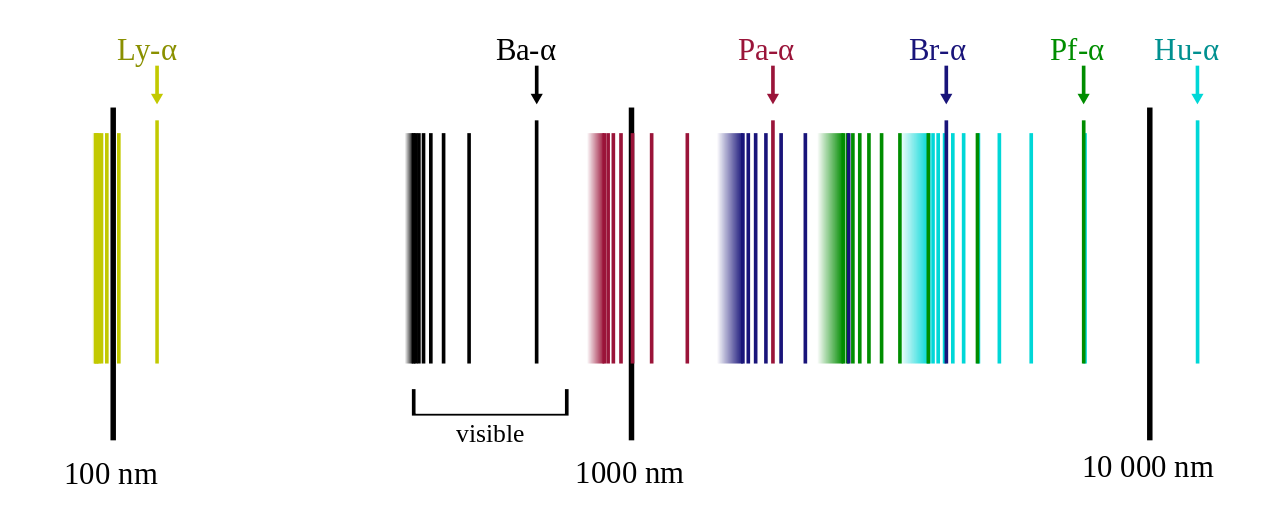
\includegraphics[width=0.4\textwidth]{hlines_wp}\newline The spectral lines of Hydrogen atom. Figure from Wikipedia.}在以下的公式中,$R_H$为常数。
        \begin{align}
          \label{eq:Blamer_line}
          \frac{1}{\lambda} = R_H \left ( \frac{1}{4} - \frac{1}{n^2}  \right )~,
          \quad n=3,4,5,\ldots
        \end{align}
        \item 1888年,里德伯:提出了氢原子的通式:
        \begin{align}
          \label{eq:Rydberg_line}
          \frac{1}{\lambda} = R_H \left ( \frac{1}{m^2} - \frac{1}{n^2}  \right )~,
          \quad n=m+1, m+2,\ldots
        \end{align}
        \item 1906年,莱曼:氢光谱的紫外波段($m=1$ of \eqref{eq:Rydberg_line}).
        \item 1908年,帕邢:氢光谱的红外波段($m=3$ of \eqref{eq:Rydberg_line}).
    }
}

如何理解元素的这样的光谱呢?像\eqref{eq:Rydberg_line}这个简易公式需要一个理论。我们需要详细理解原子与光的相互作用--了解原子内部的构造可以帮助。因此,我们继续来复习另一个研究的历史--亚原子结构。

\textbox{亚原子的发现\index{亚原子结构}}{
    原子实际上并不是物质的基础组成部分。它们是由更小的粒子组成的。
    \titem{
        \item 1897年,汤姆森:发现了电子。
        \item 1899年,卢瑟福:发现了$\alpha$粒子(氦核)。
        \item 1904年,汤姆森:原子的“葡萄干布丁”模型。
        \item 1909年,盖革、马斯登、卢瑟福:$\alpha$粒子分散。
        \item 1911年,卢瑟福:有核原子模型,就跟行星环绕太阳一样,电子沿着轨道环绕原子核。核半径约为一个原子的$10^{-5}$。
    }
    \tcblower 
    卢瑟福的原子模型有一个很严重的问题:电子在原子体积内运动肯定会有加速度。但是电荷的加速意味着E\&M辐射。电子应该会失去能量并落到原子核上。

    怎么稳定卢瑟福的原子呢?
}

光谱学和亚原子结构都已经进化到1910年代的程度了。当时物理学家开始意识到量子力学的重要性。量子力学能否解决亚原子结构的问题?又能否解释原子光谱呢?

\subsection{玻尔的氢原子模型}

\textbox{玻尔的模型\index{玻尔的原子模型}}{
    1913年,玻尔通过整合物理的三个学问建立了他的原子模型:
    \tenum{
        \item 原子光谱学:光有不同的频率:
        \begin{align}
          \label{eq:rydberg_nu}
          \nu^{(n_2, n_1)} = \frac{c}{\lambda^{(n_2, n_1)}} = c R_H 
          \left ( \frac{1}{n_2^2} - \frac{1}{n_1^2}   \right )~.
        \end{align}
        \item 光子的量子性质:光的频率是源于光子的能量: $E_\gamma^{(n_2, n_1)}=h\nu^{(n_2, n_1)}$.
        \item 亚原子结构:在氢原子里,电子可以在不同的轨道上。经典的来说,这些轨道对应电子的不同能量。首先注意力:
        \begin{align}
          \label{eq:orbit_bohr_electron}
          F = \frac{mv^2}{r} = \frac{1}{4\pi\epsilon_0}\frac{e^2}{r^2}
          \quad\Rightarrow\quad mv^2 = \frac{1}{4\pi\epsilon_0}\frac{e^2}{r}
        \end{align}
        因此电子的能量是
        \begin{align}
          \label{eq:energy_bohr_electron}
          E_e = \frac{1}{2} mv^2 + V(r) = - \frac{1}{2} m v^2~.
        \end{align}  
    }
    \tcblower
    现在我们整合这些理论。电子在轨道上的频率为$\nu_e = v / (2\pi r)$。我们可以自然地推测:如果一个电子从停在无限远到一个轨道,释放的光子的频率与电子的频率相关。
    玻尔提出
    \marginnote{这里的因数2只是个猜测,大概率是作为一个$\nu_e$和0的简易平均值。这就是电子在无限远的起始频率。不要太纠结这个因为我们马上要推翻玻尔的原子。薛定谔方程可以很清晰的算出所有东西。}
        \begin{align}
            \nu = \frac{\nu_e}{2} = \frac{v}{4\pi r}~.  
        \end{align}
    因为发射光子是被量化的,可得
    \begin{align} \label{eq:emvr}
        |E_e| = n h \nu \quad\Rightarrow\quad m v r = \frac{nh}{2\pi}~,
    \end{align}
    这里$n$为整数。用
    \eqref{eq:orbit_bohr_electron}来抵消$r$,\eqref{eq:emvr} 可以写成
    \begin{align}
        v = \frac{e^2}{2n\epsilon_0 h} \quad\Rightarrow\quad
        E_e(n) = -\frac{m e^4}{8\epsilon_0^2h^2} \times \frac{1}{n^2}~. 
    \end{align}
    这的确导出了公式\eqref{eq:rydberg_nu}:
    \begin{align}
    \nu^{(n_2, n_1)} = c R_H 
    \left ( \frac{1}{n_2^2} - \frac{1}{n_1^2}   \right )~,
    \qquad
    R_H = \frac{me^4}{8\epsilon_0^2h^3 c}~. 
    \end{align}
}

\textbox{与德布罗意物质波的关系}{
    量化条件\eqref{eq:emvr}可以被更直观地理解:把这个公式写成
    \begin{align}
        \frac{p}{\hbar} = \frac{n}{r}~,  
    \end{align}
    这里电子的动量是$p=mv$并且$\hbar = h / (2\pi)$。

    当轨道上的电子为驻波(满足周期性边界条件),我们可以发现
    \marginnote{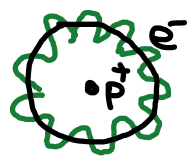
\includegraphics[width=0.15\textwidth]{bohr_atom}}
    $n/r = k$为波数。因此\eqref{eq:emvr}就是德布罗意的物质波$p=\hbar k$(提出于1924年,历史上比玻尔的原子模型晚得多)。
}

虽然玻尔的原子理论对于解释氢光谱有着很高的准确度,它无法解释氢原子的精细结构及其他多电子原子的光谱

现在我们知道了玻尔模型的失败是因为玻尔模型的半经典性质。电子的位置和动量满足不确定性原理。因此不存在经典的轨道。在考虑到完整的量子力学后,这些难题的确消失了。

\subsection{(选读)氢原子的薛定谔方程}
\label{sec:schrodinger-atom}

在这小节中,这些求解薛定谔方程的技巧为选读内容。我们将在此处不提供完整详细信息的情况下模拟该过程。

\textbox{3D 薛定谔方程}{
    在三维空间内,稳态薛定谔方程为\marginnote{这个小节中,我们用$M$来表示质量,因为传统来说$m$被用来表示磁量子数(见后面定义)。}
\begin{align}
  \label{eq:Schrodinger3d}
  \left [ 
    -\frac{\hbar^2}{2M} 
        (\partial_x^2 + \partial_y^2 + \partial_z^2)
    + V
  \right ] \psi = E \psi ~, \qquad   V \equiv V(r) \propto \frac{1}{r} ~,
\end{align}
或者是
\begin{align}
  \label{eq:Schrodinger3d1}
  (\partial_x^2 + \partial_y^2 + \partial_z^2) \psi
  + \frac{2M}{\hbar^2} (E-V) \psi = 0 ~.
\end{align}
现在我们得到一个在所有 $x,y,z$ 方向上都有导数的薛定谔方程。具有不同类型偏导数的微分方程称为偏微分方程。怎么求解呢?
}

\textbox{球坐标}{
    如果要求解这个方程,我们首先要注意到势能具有球对称性。因此球坐标更适合求解这个方程。在球坐标系中,上述方程的微分算子可以改为
\begin{align}
  \label{eq:Schrodinger3dsd}
  (\partial_x^2 + \partial_y^2 + \partial_z^2) \psi
  = \frac{1}{r^2} \partial_r (r^2\partial_r\psi)
  + \frac{1}{r^2\sin\theta} \partial_\theta (\sin\theta\partial_\theta\psi)
  + \frac{1}{r^2\sin^2\theta} \partial_\phi^2\psi ~.
\end{align}
}

\mtextbox{球谐函数}{
   其实这里的大部分过程引用已知的数学——角度方向的解可以直接写成球谐函数:$\Theta(\theta)\Phi(\phi) \propto Y_{ \ell m}(\theta, \phi)$。这个球谐函数$Y_{\ell m}(\theta, \phi)$ 已经在18-19世纪研究球面上的经典波动方程的时候被充分研究过了。但是这里我们还是用$\Theta(\theta)\Phi(\phi)$因为:
    \mtitem{
        \item 你不一定熟悉$Y_{\ell m}(\theta, \phi)$.
        \item 我们希望能打开数学的黑匣子,看看这里到底发生了什么。
    }
}
\textbox{变量分离}{
    我们要用一个叫做变量分离的技巧。这是求解一类偏微分方程的一个有力方法。我们假设解的形式为
\begin{align}
  \label{eq:separation_of_vars}
  \psi(r, \theta, \phi) = R(r)\Theta(\theta)\Phi(\phi)~.
\end{align}
薛定谔方程可以被写成
\begin{align} \label{eq:schrtp}
  & \frac{1}{R} \partial_r \left ( r^2 \partial_r R \right )
  + r^2 \frac{2M}{\hbar^2} [E-V(r)]
\nonumber\\
  +& \frac{1}{\Theta \sin\theta} \partial_\theta 
        \left ( \sin\theta \partial_\theta \Theta \right )
  + \frac{1}{\Phi \sin^2\theta} \partial_\phi^2 \Phi  = 0~.
\end{align}
这个方程有一个很有趣的结构:方程的第一行取决于$r$,而方程的第二行不取决于$r$。因此第一行也不能取决于$r$,所以$r$必须为一个常数:
\begin{align}\label{eq:schr}
  \frac{1}{R} \partial_r \left ( r^2 \partial_r R \right )
  + r^2 \frac{2M}{\hbar^2} [E-V(r)] = \ell (\ell + 1)~.
\end{align}
通过这个观察,第二行可以写为
\begin{align}
  & \frac{\sin\theta}{\Theta} \partial_\theta 
        \left ( \sin\theta \partial_\theta \Theta \right )
  + \ell (\ell + 1) \sin^2\theta
  \nonumber\\
  + & \frac{1}{\Phi}\partial_\phi^2 \Phi = 0~. 
\end{align}
这个新的方程也有类似的结构:第一行取决于$\theta$但是第二行不取决于它。因此$\theta$也是常数。我们可得
\begin{align}\label{eq:scht}
  \frac{\sin\theta}{\Theta} \partial_\theta 
        \left ( \sin\theta \partial_\theta \Theta \right )
  + \ell (\ell + 1) \sin^2 \theta = m^2~.
\end{align}
\begin{align}\label{eq:schp}
  \partial^2_\phi \Phi + m^2 \Phi = 0~.
\end{align}
这个偏微分方程可以分解为三个常微分方程:方程~\eqref{eq:schr}, \eqref{eq:scht}和\eqref{eq:schp}。常微分方程就很好解了。不过我们只会求\eqref{eq:schp}的解因为它是一个熟悉的波方程。我们会在不给太多细节的情况下给出\eqref{eq:schr}和\eqref{eq:scht}的解。
}

\textbox{欧拉函数:$L_z = m \hbar$的磁量子数$m$}{
    易证公式~\eqref{eq:schp}的解为\marginnote{一般来说,$\Phi = c e^{im\phi}$有一个常数$c$。这个常数在这里是无关紧要的所以被省略掉了。其实还有一组解$\Phi = e^{-im\phi}$。这个解相当于$m\rightarrow -m$.}
\begin{align}
  \Phi = e^{im\phi}~.
\end{align}
它们只是角方向上的左右移动波(对$z$轴来说)。物理上来说,$m$ 与角动量有关。量子力学中的角动量为$\mathbf{L} = \mathbf{r} \times \mathbf{p} = -i\hbar (r\times \nabla)$。我们可以推出在球坐标内,$L_z = -i\hbar \partial_\phi$因此,$L_z = m\hbar$。

注意波具有周期性边界条件\marginnote{这里的数学结构与玻尔的半经典原子相似。但是物理上是不一样的。我们并没有限制电子仅沿 $\phi$方向移动。我们现在只是在计算$\phi$方向的波方程。电子有几率在任何地方出现而不是仅在轨道内。}
(回想波方程的连续性):
\begin{align}
  \Phi |_{\phi=0} = \Phi |_{\phi} = 2\pi~,
  \qquad
  \partial_\phi \Phi |_{\phi=0} = \partial_\phi \Phi |_{\phi = 2\pi}~.  
\end{align}
为了满足这些条件,$m$必须是整数,也被称为磁量子数。\index{磁量子数} 
}

\textbox{$\Theta$函数:方位量子数$\ell$。}{
    现在我们来看方程\eqref{eq:scht}。我们不会在这里求解(你会在正规的量子力学课上学解法)。不过回想$\phi$方向的过程:这里有两个相似点:
\tenum{
  \item 注意$\theta$也是旋转,所以应该与某种角动量有关。因此,$\ell$应该与某种角动量有关。这个波方程的总动量为
  \begin{align}
    L^2 = \ell (\ell + 1)\hbar^2~.
  \end{align}
  \item 如果解$\Theta(\theta)$在$\theta=\pi$处为正则,$\ell$ 只能是整数。\marginnote{我们之前说了$m$与$z$方向的角动量有关、$\ell$与总角动量有关。所以我们可以很自然地理解$m$不能比$\ell$大。} $\ell$(也叫做方位量子数)\index{方位量子数}) 只能是从$m$开始的整数:$\ell = m, m+1, \ldots$我们可以这样表示这个条件:
  \begin{align}
    \ell = 0, 1, 2,3,4,5,6, \ldots~,
  \end{align}
  这些轨道在化学中被称为s、p、d、f、g、h、i$\ldots$ 。给定一个$\ell$,$m$只能是
  \begin{align}
    m = 0, \pm 1, \ldots, \pm \ell~.
  \end{align}
}
}

\needspace{0.3\textwidth}
\mtextbox{总角动量}{
    如果在势能公式中乘$\frac{\hbar^2}{2Mr^2} \ell (\ell + 1)$,这会是一个熟悉的公式。在经典力学中,在将3d中心力问题简化为1d的过程中,添加到有效势公式中的附加项是$\frac{L^2}{2Mr^2}$,$L$是电子的总角动量。与\eqref{eq:schr-alt}相比,我们可以得出结论:系统的角动量是$L^2 = \ell (\ell + 1)\hbar^2$。
}
\textbox{$R$函数:主量子数$n$\index{主量子数}}{
    我们会在不完全解的情况下,找一些公式\eqref{eq:schr} 中的感觉。我们讲公式\eqref{eq:schr}重写成
\begin{align}
    \label{eq:schr-alt}
    \frac{1}{R} \partial_r \left ( r^2 \partial_r R \right ) + r^2 \frac{2M}{\hbar^2} \left[
    \left(E - \frac{\hbar^2}{2Mr^2} \ell (\ell + 1)\right)-V(r)
    \right] = 0~.
\end{align}
这与平稳薛定谔方程相似,只不过这个的能量更少。这个能量的减少是因为我们只对化简过的一维问题感兴趣,因此必须减去来自旋转的能量。

这是一个束缚态问题。因此,能谱是离散的。解出\eqref{eq:schr-alt}后(需要技巧所以我们跳过了细节),可得
\begin{align}下·
  E = \frac{E_1}{n^2}~, \qquad 
  E_1 \equiv - \frac{m e^4}{32\pi^2 \epsilon_0^2 \hbar^2}~.
\end{align}
$n$是一个整数并且$n=\ell + 1, \ell + 2, \ldots$。这就是玻尔获得的量子化能级的结果。

很显然起始整数$n$必须被$\ell$限制因为$\ell$越大,需要从$E$扣除的角动量的能量越大。我们可以重写$n, \ell, m$的限制:
\begin{align}
  n=1,2,\ldots~, \quad
  \ell = 0, 1, \ldots, n-1~, \quad
  m = 0, \pm 1, \pm 2, \ldots \pm \ell~.
\end{align}
}

\subsection{氢原子的特质}

因为你有可能没有看上个选读的小节,这里我们概括了氢原子的特质以及它们的物理后果。

\textbox{可能的原子状态数}{
    已知$n, \ell, m$,我们可以数出可能状态的总数。这在化学中非常关键。数的时候,我们首先注意到两个关于电子的特质:
\begin{itemize}
  \item 电子是费米子,因此它们不能处于同一状态。
  \item 每组已知的$n, \ell, m$都有两个电子态。这是因为电子有自旋$m_e = \pm 1/2$,即自旋向上和自旋向下。
\end{itemize}
我们现在可以数可能原子状态的总数。比如说,当$n=1$时,我们可知$\ell =0, m=0$。因此只有两种状态(上旋和下旋)。当$n=2$,我们可得
\begin{align}
  \begin{cases}
    \ell = 0, m=0, m_e = \pm 1/2, &\quad\mbox{2种状态}\\
    \ell = 1, m=0, m_e = \pm 1/2, &\quad\mbox{2种状态}\\
    \ell = 1, m=\pm 1, m_e = \pm 1/2 &\quad\mbox{4种状态},
  \end{cases}
\end{align}
因此一共有8种状态。一般来说,已知$n$,原子会有$2n^2$种状态。

有相同$n$的电子在同一电子层上;有相同$n$和$\ell$的电子在同一轨道上。\index{电子层}\index{轨道}
}

\textbox{电子云\index{电子云}}{
    现在
    \marginnote{
    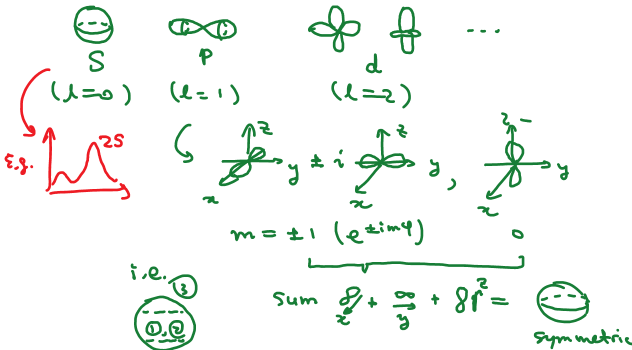
\includegraphics[width=0.4\textwidth]{e_cloud}}
    运用同样的波方程$\Psi(r, \theta, \phi)$,电子的特质用概率密度幅度表示(这种分布称为电子云)。这与经典的轨道不一样。无论如何,我们仍然可以用“轨道”来表示不同$n$、$\ell$和$m$的状态。右图显示了一些状态。

    对于每个$n$,右图显示了s, p, d, $\ldots$轨道的特征。我们可以发现无论$r$的大小,s轨道都比p和d轨道有更大的概率密度。
    
    注意它们概率密度的波动。
    \marginnote{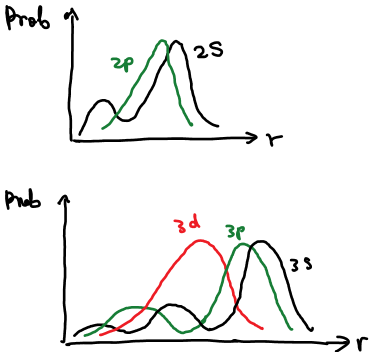
\includegraphics[width=0.35\textwidth]{spd2}}
    尽管我们我们没有明确的计算这些概率密度,我们还是可以通过我们在无限深势阱中的束缚态的经验来理解它们。
}
\textbox{转换和选择规则\index{选择规则}}{
    我们现在知道了氢原子(所有原子)可以处于确定能量的静止状态。这些状态之间也可以有转换。比如说,一个原子可以发射一颗光子来变成一个更低的能量状态;或者吸收一个光子来变成一个更高的能量状态。因为能量守恒,光子的频率是
\begin{align}
  \nu = \frac{E_{n'}-E_n}{h}~,
\end{align}
两个状态$E_{n'}$和$E_n$必须满足$\Delta \ell = \pm 1$, $\Delta m_\ell = 0, \pm 1$。因为光子的自旋为1。
}

\section{元素周期表} \label{sec:atom-multi}

现在
\marginnote{对于多电子原子来说--甚至两个电子的氦,薛定谔方程不能解析求解。你可以尝试用数值方法解决它,或者从我们对氢原子的经验中研究定性特征。}
我们想要研究除氢原子之外的元素。对于一个原子核带有$Z$ 正电荷的原子会发生什么?

\textbox{多电子原子的定性差异}{
    \titem{
        \item 泡利不相容原理:如果一个轨道被填满了,原子的其他电子会进入其他轨道。
        \item 筛选和其他电子相互作用:
        \marginnote{总体来说电子相互作用是非常复杂的。比如说从某方面来看,氦原子的电子相互作用问题就是一个量化的三体问题。幸运的是,“筛选”的观点可以给我们提供一些概念也有时是一个好的估算。}
        经典地来看,当我们考虑外层电子的运动时,内层电子会屏蔽原子核的电荷。在量子力学,没有绝对的内层、外层电子。但是在屏蔽效应中需要考虑电子的空间分布。结果,在一个氢原子里,如果$n$相同,s、p、d、f……轨道有着相同的能量。但是对于多电子原子来说,如果$n$相同,$E_s<E_p<E_d<E_f$ 因为如果角动量更大(平均来说)意味着离原子核更远,也有着更多屏蔽效应。
    }
}

我们列一些元素及它们的电子构型,从而观察这些特征是如何影响元素的电子构型的,尤其是最外面的电子层(也叫价层,是最影响化学特征的一层)。我们只会讨论它们的基态。

\textbox{元素的电子构型}{
    \titem{
        \item 氢:
        \marginnote{氢 (H, $Z=1$) \mnewline
            \begin{MOdiagram}[style=square]
                \AO{s}[label={1s}]{0;up}
            \end{MOdiagram}
        }
        氢原子的基态中,所有电子都在$n=0$状态。它只有一个s轨道($\ell = 0$)。电子有13.6 eV的电离能(原子失去电子需要的最小能量)。
        \item 氦:
        \marginnote{\newline 氦 (He, $Z=2$) \mnewline
            \begin{MOdiagram}[style=square]
                \AO{s}[label={1s}]{0}
            \end{MOdiagram}
        }   
        单纯的来看,氦的电离能应该是$Z^2 \times 13.6 \mbox{eV}= 54.4\mbox{eV}$。可是,它的电离能其实是24.5 eV。这个的原因是屏蔽效应。其实,拿走氦的第一个电子之后,我们的确需要$54.4\mbox{eV}$来拿走第二个电子(第二电离能)。

        因为氦有一个填满的价壳层,它很难给其他原子接受或者提供电子来形成化学键。因此它的化学性质非常稳定。
        \item 锂:
        \marginnote{锂 (Li, $Z=3$) \mnewline
            \begin{MOdiagram}[style=square]
                \AO{s}[label={2s}]{0;up}
                \AO(30pt){p}[label={2p}]{0.2;}
            \end{MOdiagram}
        }
        它有3个电子,所以一个电子必须在$n=2$电子层。那个电子会去2s($\ell=0$)轨道还是2p($\ell=1$)轨道呢?根据屏蔽效应,s轨道能量更低所以电子会去s轨道。锂的电离能是5.45 eV。它很容易就能失去这个电子,因此锂有一个活性化学性质。
        
        \item 从铍到氩,我们继续填进2s, 2p, 3s, 3p轨道。
        
        \item 钾
        \marginnote{钾 (K, $Z=19$) \mnewline
            \begin{MOdiagram}[style=square]
                \AO{p}[label={3d}]{0;}
                \AO(60pt){s}[label={3d}]{0;}
                \AO(80pt){s}[label={3d}]{0;}
                \AO(110pt){s}[label={4s}]{-0.2;up}
            \end{MOdiagram}
        }
        天真的来看,我们会去填3p之后的3d。但是,因为3d轨道的角动量太大了,它的能量比4s稍微多一点。所以钾的4s轨道会先被填。
    }
}

\needspace{0.1\textwidth}
希望上面的讨论能给你一些对于元素周期表的了解。\index{元素周期表}
\marginnote{\begin{center}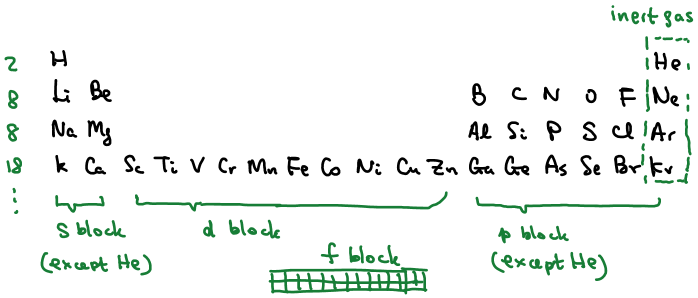
\includegraphics[width=0.35\textwidth]{ptab}\end{center}}

\section{结语:总结与未来}

\textbox{额外参考阅读}{
    \titem{
        \item 关于原子大小的更多细节可以在 \href{http://www.informationphilosopher.com/solutions/scientists/maxwell/illustrations_dynamical_theory_gases_1.pdf}{麦克斯韦}和 \href{https://www.chemteam.info/Chem-History/Loschmidt-1865.html}{洛施密特}的原作里找到。麦克斯韦的论文有更多技术计算,而洛施米特的论文可以更容易的理解。
        \item 虽然玻尔的原子模型被薛定谔方程法超越了,但是如果你仍对历史上的细节感兴趣,你可以看看 \href{http://hermes.ffn.ub.es/luisnavarro/nuevo_maletin/Bohr_1913.pdf}{玻尔的原论文}。
        \item 关于薛定谔方程和元素周期表的细节可以在 \href{http://www.feynmanlectures.caltech.edu/III_19.html}{费曼讲座III章节19}被找到。关于更多化学上的细节,你可能会想要读一本关于物理化学的书,比如说 \href{https://www.amazon.com/Physical-Chemistry-Robert-J-Silbey/dp/047121504X}{锡尔贝、阿尔伯蒂、巴文迪的《物理化学》}。
    }
}

\textbox{下一步是什么?}{
    这个章节的量子部分会在量子力学和物理化学中被更深的研究。

    物质的原子和亚原子结构只是一个研究内部物质结构的起点,而不是一个结束。粒子物理会对基本粒子有更深的研究。我们也会在之后的章节--粒子和弦里继续接触粒子物理的细节。
}


\section{练习题}

\textbox{E\wref{sec:atom-hydrogen}.1 来自物质波的玻尔原子}{
    玻尔的假设$\nu=\nu_e/2$看上去很神秘。不用这个假设,而用德布罗意的物质波和其他玻尔模型的假设来推导$R_H$。
}

\textbox{E\wref{sec:atom-hydrogen}.2 原子态}{
    对于一个氢原子:
    \tenum{
        \item 主量子数为$n=3$,有多少个电子态?
        \item 在这些$n=3$的状态中,有多少个状态分别在$s$、$p$和$d$轨道?
        \item 设$n=3$状态的能量为$E_3$。现在,由于过渡演化(即 $n=3$ 是初始或最终状态)$n=3$状态而发射光子。求光子尽可能最大的频率,用$E_3$和普朗克常数$h$表示?(注意:你不必考虑原子的精细和超精细结构。)
    }
}

\textbox{E\wref{sec:atom-multi}.1 电子排布}{
    求Be、C、Ne和K的电子排布。
}

\printindex

\end{document}